\documentclass{article}
\usepackage[code]{qjpzh}
\usepackage[scale=0.75]{geometry}
\title{毕设工程说明文档}
\author{\qjp}
\date{}
\begin{document}
\maketitle
\section{工程概况}
毕设的工作共有两个工程,分别为TemplateExtractor和TemplateExtractorDemo,实现语言
都是Scala,开发环境为Eclipse。其中,Scala的版本为2.10.1,由于Scala本身不向后兼容,
因此必须保证所有的代码都采用同一版本进行编译。所有的程序仅保证可以在Linux下运行。

注:很多Linux发行版的仓库中的Scala主版本号还是2.9(如我使用的Ubuntu 13.04),因
此我是手动安装的Scala 2.10。

我在我的服务器账号qiujunpeng目录下手动安装了需要的软件,并配置好了环境变量,因此
使用qiujunpeng账号登陆可以直接使用各个软件。

TemplateExtractor为主要的工程,实现了模板的自动聚类和抽
取;TemplateExtractorDemo比较简单,实现了模板匹配的演示Web Service。
\section{TemplateExtractor介绍}
\label{sec:templateextractor}
\subsection{代码管理综述}
\newcommand*{\prj}{PROJECT\_DIR}
代码的编译和管理采用SBT(Simple Build Tool),是类似Java的Maven的一个代码自动构建工
具,详细的介绍可以看\url{http://www.scala-sbt.org/}。SBT的主要配置文件
为build.sbt,置于工程根目录下,下面以\prj表示项目的根目录。所有工程中的依赖关系,
即用到的所有第三方库,包括twitter util,akka,jsoup,icu4j等都统一使用SBT进行管理。
使用的SBT版本为0.12.0。

\subsection{SBT使用方法}
\label{sec:sbt}
以下说明SBT的使用方法:
\begin{itemize}
\item 编译、运行代码:修改根目录\prj下的build.sbt中的最后一行:\\
  \coding{scala}{mainClass in (Compile, run) := Some("path.to.main.class")}
  将其中的\texttt{path.to.main.class}修改为需要运行的类的路径。在根目
  录\prj键入\icoding{sbt}命令,即可进行SBT的控制台。在SBT的控制台中,输
  入\icoding{compile}编译,然后输入\icoding{one-jar}导出为Jar包(需要安
  装SBT的sbt-onejar插件,工程地址为\url{https://github.com/retronym/sbt-onejar})。
  进入SBT的控制台后,输入\icoding{one-jar}即可导出Jar包。导出的Jar包有两个:\\  
  \begin{code}{sh}
PROJECT_DIR/target/scala-2.10/templateextractor_2.10-0.1-SNAPSHOT.jar  
PROJECT_DIR/target/scala-2.10/templateextractor_2.10-0.1-SNAPSHOT-one-jar.jar
  \end{code}
  第一个包含工程所有的源代码编译成的.class文件,第二个则包含了第一个Jar包和所有的
  依赖库(包括Scala标准库和我们使用的所有第三方库),因此第二个Jar包实际上和普通
  的Java程序导出的Jar包是一样的,可以像Java程序导出的Jar包一样直接执行:\\
  \coding{sh}{java -jar templateextractor_2.10-0.1-SNAPSHOT-one-jar.jar}
\item 导出Eclipse工程:为了使用Eclipse进行开发,需要将SBT工程导出为Eclipse工程。
  安装SBT的sbteclipse插件后,在SBT控制台输入\icoding{eclipse}即可导出Eclipse工程。\\
  有一点需要注意,使用sbteclipse导出成Eclipse工程时,原来SBT工程中的资源文件目录
  不会加入到导出工程的classpath中。代码中使用了typesafe的config库管理和读取配置文
  件,配置文件application.conf放在\prj/conf下。为了使config库可以正确找到配置文件,
  需要在\prj/build.sbt中将\prj/conf加入到SBT工程的资源文件目录中,而使
  用sbteclipse导出时该目录将不会出现在导出的Eclipse工程的classpath中,此时如果直
  接运行导出后的Eclipse工程,config库将无法找到配置文件。因此在使
  用sbteclipse导出Eclipse工程后,还需要在Eclipse中手动将\prj/conf目录加入到''Build
  Path''中。
\item 安装SBT插件:工程中安装了sbt-onejar和sbteclipse两个插件,使
  用\icoding{addSbtPlugin}函数安装插件,见\prj/project目录里的build.sbt文件(不是
  根目录\prj下的build.sbt)。
\end{itemize}
\subsection{一些shell脚本}
从第~\ref{sec:sbt}节中可以看到,编译、运行一次代码需要很多步骤,手动操作的话很麻
烦。另外,目前Scala编译器编译的速度比较慢,在实验室台式机上编译一次整个工程需
要3分钟的时间(我的笔记本配置好一些,但也要1分钟左右)。因此,为了编译和调试代码
方便,我写了一些shell脚本简化这些步骤,都放在了\prj/tools目录下。这些脚本本身都非
常简单易懂,下面仅对主要的脚本进行说明:
\begin{itemize}
\item \texttt{rsync\_source.sh}:Scala编译器可以有效使用多个线程同时编译,因此放
  到服务器上可以大大加速编译速度。在服务器上的实测结果是编译整个工程只需要10s左右
  的时间。这个脚本的作用是利用rsync将全部代码同步到服务器上,以便在服务器上可以进
  行代码的编译。该脚本一般不直接使用,而是被其他的脚本调用。
\item \texttt{make\_jar.sh}:程序的开发和调试放在本地,运行则在服务器上,因此需要
  准备两个不同的配置文件。\prj/conf目录下有两个文
  件:application.conf和application.conf.server,分别用于本地和服务器上的配
  置。config库默认使用application.conf作为配置文件,在本地调试的时候这是没有问题
  的,如果要在服务器上运行时则需要更换配置文件。这个脚本的作用即是在导出成服务器
  上运行的Jar的时候设置application.conf.server为配置文件,并根据用户的输入自动修
  改\prj/build.sbt中类的路径,编译并打包成可运行的Jar包。这个脚本也不直接使用,
  而是被其他脚本调用。
\item \texttt{send\_server.sh}:这是主要使用的脚本。先调
  用\texttt{rsync\_source.sh}自动将整个工程同步到服务器,然后调
  用\texttt{make\_jar.sh}在服务器上编译并导出成Jar包,之后运行该Jar包。脚本接受一
  个参数,该参数为需要运行的类的路径。使用方法示
  例:\\\coding{sh}{tools/send_server.sh
    thu.ailab.template.TestTemplateManager}
\item \texttt{send\_client.sh}:这个脚本和\texttt{send\_server.sh}的作用和使用方
  法都一样,唯一的不同是这个脚本没有和服务器之间同步代码,而是在本地编译打包完后
  将最后导出的可运行的Jar包上传到服务器上。如果需要在本地进行编译,则使用这个脚本
  代替\texttt{send\_server.sh}。实际开发过程中我都是用\texttt{send\_server.sh},
  没有使用这个脚本,因为本地的编译速度太慢了。
\item  \texttt{fix\_template.sh}:这个脚本将服务器生成的模板XML文件转化为本地使
  用的模板XML文件。主要的作用是供另外一个工程TemplateExtractorDemo使用。
\end{itemize}

\subsection{代码运行说明}
\label{sec:code}
之前已经介绍完了代码的管理,接下来说明如何运行程序。

程序分成多个模块,每个模块单独运行,前一个模块运行完了以后将结果输出成文本文件或
者XML,下一个模块读取这些文件恢复状态。所有的模块都可以通
过\texttt{send\_server.sh}来运行,比如预处理模块:\\\coding{sh}{send_server.sh thu.ailab.document.TestDocProcessor}

由于实验有几个不同的数据集,因此需要设定目前程序在那个数据集上运行,修
改\prj/conf下的配置文件中的\texttt{global.dataset}即可,目前的取值可以
为\texttt{blog}或\texttt{news}。为了叙述方便,下面将用\texttt{DATASET}指代某个具
体的数据集。

按顺序依次运行以下几个主要模块:
\begin{itemize}
\item 预处理:对应的类的路径为\texttt{thu.ailab.document.TestDocProcessor}。运行
  该类后,原始的HTML文档将经过去除多余标签、遍历成序列、去除重复记录等步骤,最后,
  预处理后的文档将保存到另外一个目录中。
\item 计算文档相似度:对应的类的路径为
  \texttt{thu.ailab.distance.TestDocDistance}。运行该类后将计算所有输入文档两两
  之间的距离,并将距离保存到文本文件中。
\item 文档聚类:对应的类的路径
  为\texttt{thu.ailab.cluster.TestDocNaiveAggloCluster}。运行该类后将进行聚类,
  将聚类结果输出为XML。
\item 模板生成:修改配置文件application.conf中的\texttt{global.stage},将值改
  为\texttt{build},然后再用\texttt{send\_server.sh}运行,对应的类的路径
  为\texttt{thu.ailab.template.TestTemplateManager}。运行后将生成一个模板的XML文
  件。
\item 模板标注:对应的类的路径仍
  为\texttt{thu.ailab.template.TestTemplateManager}。同样需要修改配置文
  件application.conf中的\texttt{global.stage},将值改为\texttt{extractRandom}。修
  改后运行程序,将随机抽取测试集中的某个样本,然后利用模板进行抽取。根据抽取的结
  果,决定我们真正需要的字段是哪些,然后对生成的模板XML文件中对应的部分进行标注。
  标注的类型在thu/ailab/template/ExType.scala中定义,可以根据需要往其中手动添加,
  目前有\texttt{TITLE,CONTENT,AUTHOR}三种,\texttt{MAGIC}类型表示没有标注。自动生
  成的模板XML中默认所有的标签的\texttt{exType}值都为\texttt{MAGIC}。下面举个例子:
  当我们决定某个div标签对应的为
  \texttt{CONTENT}时,我们修改XML:\\
  \begin{code}{xml}
<treenode allowMultiple="false" exType="MAGIC">
      <names>
      <name>div</name>
      </names>
      <depths>
      <depth>9</depth>
      </depths>
</treenode>    
  \end{code}
  中的\texttt{exType}属性,将其改为\texttt{CONTENT},如下所示:\\
  \begin{code}{xml}
<treenode allowMultiple="false" exType="CONTENT">
    <names>
    <name>div</name>
    </names>
    <depths>
    <depth>9</depth>
    </depths>
</treenode>
  \end{code}

  这样模板标注就完成了。
\item 内容抽取:对应的类的路径还
  是\texttt{thu.ailab.template.TestTemplateManager}。需要修改配置文件中
  的\texttt{global.stage}为\texttt{extractAll}。从测试集中抽取的文件个数可以修改
  配置文件中的\texttt{DATASET.template.extractCount}。抽取的结果将被保存为XML文件,
  文件路径由\texttt{DATASET.\\template.extractResult}决定。
\end{itemize}

\subsection{配置文件说明}
程序的正常运行非常依赖于配置文件。配置文件中的一些键值是程序运行的参数,如聚类的
阈值,Actor的个数等;另外很大一部分是程序输出文件路径的配置,如保存文档集合两两之
间距离的文件路径,保存模板XML的文件路径等等,这里不一一列举说明,每个文件路径的具
体含义可以参考代码中对应的使用到这些量的地方。文件路径中可以
用\texttt{\textasciitilde{}}表示用户的家目录。

\section{TemplateExtractorDemo介绍}
\label{sec:templ}

\subsection{Play! 框架介绍}
\label{sec:play}
这个Web Service采用Play! Framework实现,网址为\url{playframework.org},Play的版本
号为2.1.1,该版本依赖的Scala版本为2.10。Play目前仍处于活跃开发中,不同版本有不兼
容的情况,因此必须保证版本号一致。

Play的工程底层采用SBT进行管理,使用方法上和SBT很类似。下载并配置好了Play之后,在
命令行使用\icoding{play}进入到Play的控制台,这个控制台和SBT的控制台差不多,不过
增加了一些命令。输入\icoding{run}即可在本地的9000端口运行我们的Web Service。

\subsection{Web Service使用说明}
下面使用\prj表示项目的根目录。为了正确运行程序,需要的文件有TemplateExtractor工程
导出的Templateextractor\_2.10-0.1-SNAPSHOT-one-jar.jar文件和TemplateExtractor工程
依赖的包。可以使用第~\ref{sec:templateextractor}节中介绍的方法导
出templateextractor\_2.10-0.1-SNAPSHOT-one-jar.jar,然后复制该Jar包到\prj/lib中,
或者通过运行\prj/tools/retrieve\_txjar\_local.sh来自动完成编译、导出和复制的工
作。TemplateExtractor工程所依赖的包(jsoup,icu4j等)也需要加入到Play工程的依赖中,
依赖定义在文件\prj/project/Build.scala中。

Play的配置文件为\prj/conf/application.conf,需要向其中增
加
\texttt{cluster.\\DocNaiveAggloCluster.clusterThreshold,templateFiles.blog,templateFiles.news}
三个值,后两者分别用于指定blog数据集和news数据集的标注好的模板文件的路径。

Web Service的路径定义在\prj/conf/routes中,定义了4种路径,分别为:\\
\begin{code}{sh}
/blog/l/*url
/news/l/*url
/blog/w/*url
/news/w/*url  
\end{code}
/blog和/news前缀表示匹配那种数据集的模板,中间的l和w分别表示local和web,最后
的*url表示需要进行模板匹配的文件的url。前两个中的url必须是本地路径,
以\texttt{/}开头;后两个中的url必须是Web上的一个url,以\texttt{http://}开头。前两
个路径可以正常使用,只需要将*url部分替换为一个本地测试HTML文件的地址即可;而后两
个路径暂时存在一些问题:由于目前用于训练的文件是之前的同学已经抓取好的网页,
和Web上直接得到的有些不同,匹配时有一些差错,测试发现后两个路径暂不能正常使用。

需要注意的是,由于模板的XML文件是在服务器上生成的,而目前的Web Service则是在本地
运行,因此需要将该模板XML中一些和路径相关的东西进行转化,即将服务器上的相关路径和
文件转化为本地的路径和文件。在TemplateExtractor工程根目录下的tools目录里有一
个\texttt{fix\_template.sh}shell脚本负责这个转化。这个脚本接受一个参数,该参数为
服务器生成的模板文件的路径,详细的实现可以参考该脚本的具体内容。

运行这个Web Service的步骤很简单,在Play控制台输入\icoding{run}之后,访
问localhost:9000对应的路径即可。示例:在浏览器中访
问
http://localhost:9000/blog/l//home/qjp/Programs/BachelorThesis/Data/blog1000/\\http\%3A\%2F\%2Fblog.sina.com.cn\%2Fs\%2Fblog\_000612600100y7ne.html
,http://localhost:9000/blog/l/后面的url部分是我本地的某个测试文件的地址,可以得到\\
\begin{figure}[h]
  \centering
  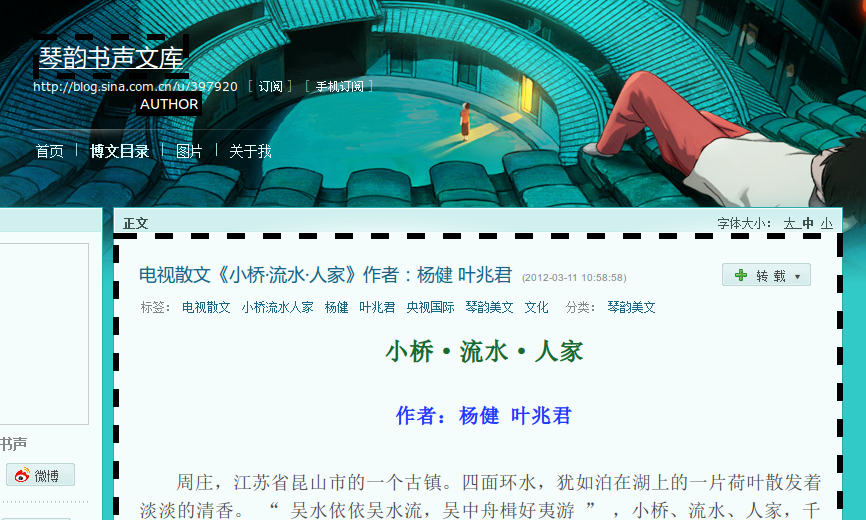
\includegraphics[width=0.8\linewidth]{demo}
\end{figure}
\end{document}